\section{Grundlagen}
\label{sec:basics}

\subsection{Arten von VR Headsets}
\label{sec:vr-headset-types}

Bei VR Headsets werden grundsätzlich drei verschiedene Arten unterschieden:

\begin{itemize}
    \item Tethered Headsets
    \item Standalone Headsets
    \item Smartphone und Handheld Headsets
\end{itemize}

In Folge werden diese Arten kurz beschrieben, sodass die beschreibungen von der Technologien verstanden werden können.
Für eine genauere beschreibung dieses Themas wird auf~\cite{ANIWAA_TEAM_2021} verwiesen.

\emph{Tethered VR Headsets} müssen immer mit einem Computer verbunden sein, weil die VR-Applikation ausschließlich auf dem Computer läuft.
Die Brille hat dabei einerseits die Funktion die vom Computer gerenderten daten darzustellen und andererseits Positionsdaten an den Computer zurückzusenden, damit diese in der Applikationslogik verwendet werden können, um zukünftige Bilddaten zu rendern.

Bei \emph{Standalone VR Headsets} ist in der Brille ein Computer integriert, auf welchem die VR Applikation läuft.
Der Computer dient ausschließlich aus Entwicklungsplattform und die fertigen Applikationen müssen auf die Brille heruntergeladen werden.

Im Falle des \emph{Smartphone VR Headsets} läuft die Applikation auf einem Smartphone.
Um die Immersion zu erhöhen wird das Smartphone in die VR-Brille eingeschoben.
In diesem Fall dient das Telefon sowohl als Anzeigegerät als auch als Sensordatenprovider.
Die VR-Brille besteht ausschließlich aus Linsen welche die Immersion der am Handy laufenden Applikation erhöht.

\subsection{Tracking}
\label{sec:tracking}

Unter Tracking versteht man das ermitteln der Position von Objekten in der realen Welt.
Folgend werden Arten das Tracking beschrieben.
Diese beinhalten:

\begin{itemize}
    \item Outside In Tracking
    \item Markerless Inside Out Tracking
    \item Marker Based Inside Out Tracking
\end{itemize}

Wie im vorigen Abschnitt wird hier nur ein Überblick über diese Arten des Trackings gegeben.
Für nähere Informationen wird auf~\cite{Dennis_Ziesecke_2019} verwiesen.

\emph{Outside In Tracking} beschreibt das Ermitteln der Positionen durch außenstehende Sensoren.
Das bedeutet, dass das zu trackende Objekt nicht weiß wo es sich im Raum befindet (Es ist passiv).
Währenddessen ermitteln außenstehende Sensoren die Position der zu trackenden Objekte und gibt diese an die VR-Applikation weiter.

Im Gegensatz dazu gibt es das \emph{Inside Out Tracking}.
Hier ermitteln Sensoren, welche sich auf den Objekten befinden die Position derselbigen.
Dabei gibt es zwei verschiedene Arten, welche bereits oben aufgelistet worden sind.

Im Fall von \emph{Markerless Inside Out Tracking} wird natürliches Licht verwendet.
Typischerweise werden hierbei Kameras verwendet.
Die dabei aufgenommenen Bilder werden mithilfe von Bildverarbeitungsmethoden analysiert und somit wird die Position der Objekte ermittelt.

Bei \emph{Marker Based Inside Out Tracking} wird im Gegensatz kein natürliches Licht verwendet.
Hierbei ist sind die zu trackenden Objekte von Lighthouses (siehe Abschnitt~\ref{sec:lighthouse_tracking}) abhängig.
Diese beleuchten den Raum mit nicht sichtbaren licht welches von Fotosensoren an den Geräten empfangen wird.

\section{VR Headset}
\label{sec:vr-headset}
\setauthor{Quirin Ecker}

Es sind einige VR Headsets auf dem Markt.
Nach einer Statistik aus 2017 sind die beliebtesten VR Headset Hersteller Sony, Oculus und HTC (Siehe Abb.~\ref{fig:vr_headset_manufacturer_marketshare}).
Folgend sind 3 VR Brillen beschrieben.
Hierbei wurden die auf die Spielkonsolen-basierten VR Headsets nciht berücksichtigt.

\begin{figure}
    \centering
    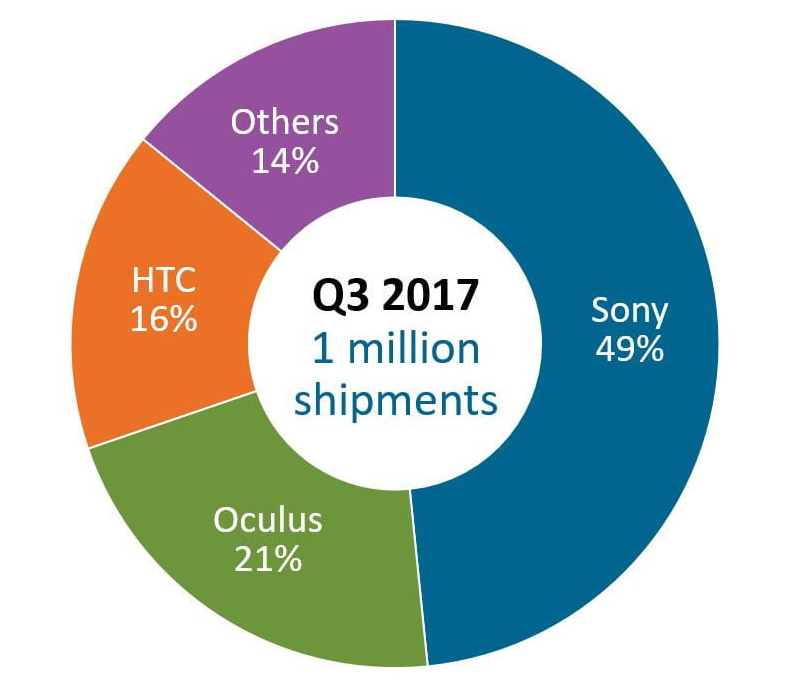
\includegraphics[scale=0.25]{pics/vr_headset_manufacturer_marketshare}
    \caption{Market-share VR Headset Hersteller~\cite{MARTINDALE_2017}}
    \label{fig:vr_headset_manufacturer_marketshare}
\end{figure}

\subsection{HTC Vive Pro}\label{sec:htc-vive}

Wie bereits in Abschnitt~\ref{sec:vr-headset-types} beschrieben, gibt es von diesen Headsets verschiedene Modelle.
Die HTC Vive Pro ist vom Typ ein tethered Headset mit dem Zusatz, dass auch sogenannte Light Houses gebraucht werden (siehe Abschnitt~\ref{sec:lighthouse_tracking}).
Andere Produkte, wie die im Folgendem beschriebene Oculus Quest benötigen solche nicht~\cite{MECHATECH}.

\subsubsection{Vorteile}

\begin{itemize}
    \item \textbf{SteamVR Verwaltung:} Die HTC kann mit SteamVR verwaltet werden, womit der manuelle Download von externer Software vermieden wird.
    \item \textbf{Lighthouse Tracking:} Zum Zeitpunkt des Verfassens dieser Arbeit ist Lighthouse Tracking verglichen mit anderen Tracking-Methoden die genaueste.
    Aus Abbildung~\ref{fig:tracking_precision_statistic} kann entnommen werden, dass das Valve Lighthouse Tracking die kleinsten Abweichungen in allen drei Dimensionen hat.
    Ein weiterer Vorteil des Lighthouse Tracking ist, dass kein natürliches Licht für den Tracking Process gebraucht wird~\cite{Dennis_Ziesecke_2019}.
    Details zum Thema Lighthouse Tracking können im Abschnitt ~\ref{sec:lighthouse_tracking} entnommen werden.
\end{itemize}

\begin{figure}
    \centering
    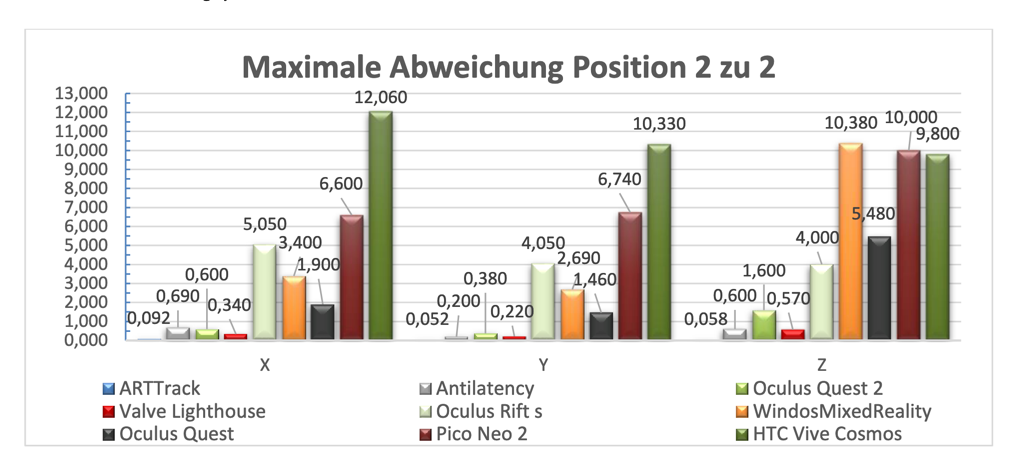
\includegraphics[scale=0.4]{pics/tracking_precision_statistic}
    \caption{Tracking Genauigkeit der VR Headsets~\cite{Macedo_2020}}
    \label{fig:tracking_precision_statistic}
\end{figure}

\subsubsection{Nachteile}

\begin{itemize}
    \item \textbf{Komplizierterer Aufbau:} Durch die Notwendigkeit der Base Stations, welche für das Lighthouse Tracking gebraucht werden, ist der Aufbau komplizierter.
    Die Base Stations müssen etwas erhöht sein, weshalb ein Stativ oder sogar eine Wandmontage notwendig ist.
    Außerdem müssen die Base Stations die zu trackenden Geräte im Sichtfeld haben.
    Für weitere Informationen wird auf den Abschnitt~\ref{sec:lighthouse_tracking} verwiesen.
    \item \textbf{Hoher Preis:} Nach der Erhebung, welche in Abb.~\ref{fig:vr_headset_prices} zu sehen ist, befindet sich die HTC Vive Pro im oberen Preissegment.
    \item \textbf{Tethered:} Wie bereits in Abschnitt~\ref{sec:basics} beschrieben worden ist, benötigen tethered Headsets eine permanente Verbindung zu einem Computer.
    Das bedeutet einerseits, dass der Transport komplizierter ist und für Normalverbraucher, ohne einen leistungsstarken Computer, der Preis für das Gesamtsystem steigt.
    Besonders der Transportaspekt ist für diese Arbeit kritisch, da diese an vielen Plätzen hergezeigt werden soll.
\end{itemize}

\begin{figure}
    \centering
    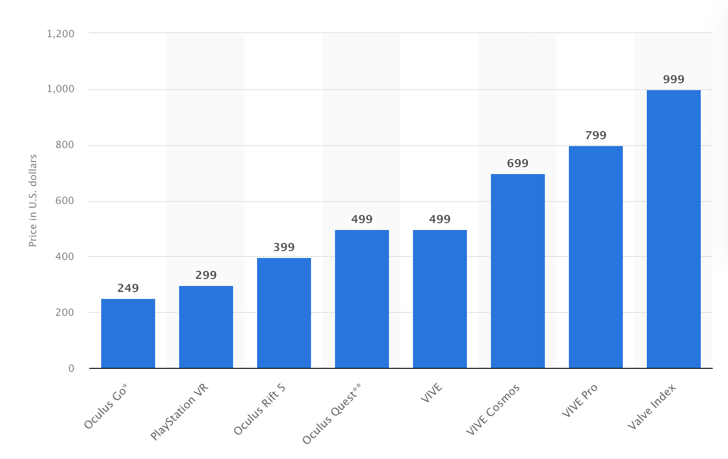
\includegraphics[scale=0.5]{pics/vr_headset_price_statistic}
    \caption{VR Headset Preise~\cite{ALSOP_2019}}
    \label{fig:vr_headset_prices}
\end{figure}

\subsection{Valve Index}

Die Valve Index ist eine VR-Brille welche von Valve entwickelt worden ist.
Diese befindet sich genauso wie die HTC Vive Pro~\ref{sec:htc-vive} im teureren Spektrum~\cite{ALSOP_2019} der VR-Brillen und ist dem Typ tethered Headset~\ref{sec:vr-headset-types} zuzuordnen.

\subsubsection{Vorteile}

\begin{itemize}
    \item \textbf{Hand Tracking}: Valve benützt bei ihren Controllern einen speziellen Entwurf.
    Die Controller besitzen eine Lasche, welche an dem Griff des Controllers hängt.
    Diese Lasche hält den Controller and der Hand, auch wenn diese den Controller nicht festhält.
    Mit dieser Technik kann der Controller losgelassen werden und die Finger frei bewegt werden.
    Um diese Finger auch in die virtuelle Welt zu übertragen, benützen die Controller Sensoren, welche an diesen angebracht sind.
    Die Informationen der Fingerpositionen können daraufhin von Entwicklern in ihren Spielen benutzt werden.~\cite{SadlyItsBradley_2019}.
    Werden diese nicht benutzt, steht trotzdem noch die normale Controller Steuerung zur Verfügung.
    \item \textbf{Lighthouse Tracking}: Die Valve Index benützt genauso wie die HTC Vive Pro das Lighthouse tracking mit dem Unterschied, dass beide Versionen des Lighthouse Tracking verwendet werden können.
    Für mehr Informationen wird auf~\ref{sec:lighthouse_tracking} verwiesen.
\end{itemize}

\subsubsection{Nachteile}

\begin{itemize}
    \item \textbf{Komplizierter Aufbau:} Genauso wie bei der HTC Vive Pro ist der Aufbau etwas komplizierter, da das Lighthouse Tracking~\ref{sec:lighthouse_tracking} verwendet wird.
    \item \textbf{Hoher Preis:} Noch teurer, wie die zuvor genannte HTC Vive Pro ist die Valve Index.
    Dies ist in der Abb.~\ref{fig:vr_headset_prices} ersichtlich.
    \item \textbf{Tethered:} Wie bereits zuvor beschrieben ist auch die Valve Index ein tethered Headset.
    Somit braucht auch diese eine permanente Verbindung zu einem Computer.
    FÜr mehr Informationen wird auf Abschnitt~\ref{sec:vr-headset-types}
\end{itemize}

\subsection{Oculus Quest 2}\label{sec:oculus-quest-2}

Die Oculus Quest 2 ist eine VR-Brille welche von Facebook/Meta im Jahre 2020 entwickelt worden is~\cite{ADI_ROBERTSON_2020}.
Diese Brille ist eine Mischung von einem tethered Headset und einem Standalone Headset~\ref{sec:vr-headset-types}.
Dies bedeutet, dass die Oculus Quest 2 ohne einen Computer benutzbar ist, aber auch mit einem USB-C Kabel zu einem Computer verbunden werden kann.
Ist das Headset mit dem Computer verbunden können PC exclusive Spiele mit der Oculus Quest 2 auch gespielt werden~\cite{ADI_ROBERTSON_2020}
Für den Aufbau werden nur das Headset und zwei Controller benötigt.

\subsubsection{Vorteile}

\begin{itemize}
    \item \textbf{Einfacher Aufbau:} Im Gegensatz zu den zuvor genannten VR-Brillen benötigt die Oculus Quest 2 kein Lighthouse Tracking verwendet.
    Dies hat einen einfacheren Aufbau zur Folge, da keine Basistationen aufgebaut werden müssen.
    Zum Aufbau werden lediglich die Brille, die Controller und eventuell noch ein Computer verwendet, wenn die Oculus Quest im tethered Modus gebraucht wird~\cite{MECHATECH}.
    \item \textbf{Günstiger Preis:} Die Oculus Quest ist im Vergleich zu den zuvor genannten Brillen eine günstigere Alternative.
    Dennoch gibt es noch günstigere VR-Headsets auf dem Markt.
    Für nähere Einsicht wird auf die Abb.~\ref{fig:vr_headset_prices} verwiesen.
    \item \textbf{Standalone:} Wie bereits beschrieben ist die Oculus Quest 2 eine Mischung aus tethered und standalone Headset.
    Kein Computer wird benötigt unter der Voraussetzung, dass auf die Leistung des Computers verzichtet werden kann.
    Für mehr Information wird auf Abschnitt~\ref{sec:vr-headset-types} verwiesen.
\end{itemize}

\subsubsection{Nachteile}

\begin{itemize}
    \item \textbf{Lichtabhängigkeit:} Durch das kamera-basierte Tracking-system~\ref{sec:oculus_quest_tracking} ist die Oculus Quest 2 von dem natürlichen Licht abhängig~\cite{Dennis_Ziesecke_2019}.
    Dieses Problem wurde von den zuvor genannten VR-Brillen durch das Licht der Basistationen gelöst~\ref{sec:lighthouse_tracking}\cite{Dennis_Ziesecke_2019}.
    \item \textbf{Full Body Tracking:} Die HTC Vive Tracker, welche üblicherweise für das Full Body Tracking verwendet werden, funktionieren mit dem Lighthouse Tracking~\ref{sec:lighthouse_tracking}.
    Da die Oculus Quest 2 diese Trackingmethode nicht verwendet kann das Full-Body-Tracking etwas komplizierter werden.
    Für verschiedene Möglichkeiten Full Body Tracking trotzdem zu erreichen wird auf~\cite{Martin_Rakver} verwiesen.
    \item \textbf{Tracking:} In Abb.~\ref{fig:tracking_precision_statistic} ist ersichtlich, dass das Tracking der Oculus Quest 2 schlechter abschneidet wie das der zuvor genannten Brillen.
\end{itemize}

\section{Lighthouse Tracking}\label{sec:lighthouse_tracking}

\subsection{Grundlagen}

Die HTC Vive Brillen und die Valve Index benützen beide das Lighthouse-Tracking~\cite{steam_lighhouse_versions}.
Diese Form des Trackings ist genauso wie das Tracking der Oculus Quest und Oculus Quest 2 (siehe~\ref{sec:oculus_quest_tracking} und~\ref{sec:oculus-quest-2}) ein Inside-Out Tracking.
Im Gegensatz zu der Oculus Quest benützt das Lighhouse Tracking kein natürliches Licht, sondern für das Auge unsichtbares Licht.
Diese Form des Tracking wird auch Marker-Based Inside-Out Tracking genannt\ref{sec:tracking}.
Im Falle des Lighhouse Tracking beleuchten die Base Stations die zu trackenden Geräte, womit sich die Geräte orientieren können.
Dies hat den Vorteil, dass die Benutzung der Vr Brille nicht von dem natürlichen abhängig ist.
Statt Kameras besitzt ein zu trackendes Gerät Fotosensoren~\cite{Buckley_2015}.

\subsection{Positionierung}

Damit dieser Vorgang fehlerfrei funktioniert werden typischerweise zwei Basestations verwendet
Diese werde wie in Abb~\ref{fig:basetstation_positioning} positioniert.
Mögliche Fehler können auftreten, wenn die Lighthouses keine klare Sicht auf die Geräte haben~\cite{steam_lighhouse_versions}..

\begin{figure}
    \centering
    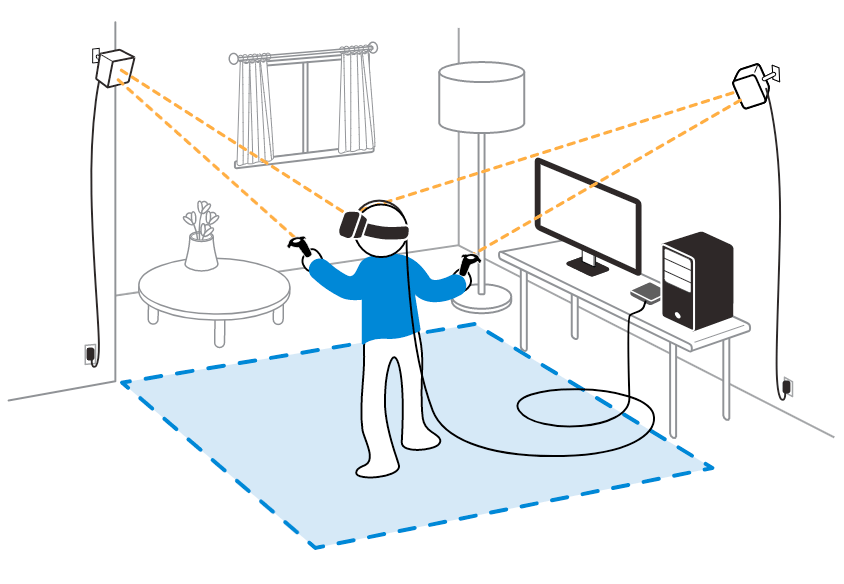
\includegraphics[scale=0.4]{pics/basestations_positioning}
    \caption{Positionierung der Lighhouses~\cite{Sercan_2018}}
    \label{fig:basetstation_positioning}
\end{figure}

\subsection{Funktionsweise}

Die Base Station besteht aus Syncblinker und Laseremitter.
Der Syncblinker ist ein Infrarot Strahl und die anderen 2 Laseremitter sind Lichtstrahlen welche sich 60-mal in der Sekunde auf einer Drehscheibe drehen.
Um die Position zu ermitteln, flasht der Sync Blinker und sobald dieser bei der Brille ankommt, fängt das Gerät zu zählen an bis die Lichtstrahlen der Laseremitter ankommen.
Durch die Drehscheibe, auf der sich die Laseremitter befinden, beleuchtet die Base Station so viele wie mögliche Sensoren.
Die Position mehrerer Punkte des Gerätes ist somit bekannt und es kann die Rotation der Brille ebenfalls berechntet werden~\cite{Buckley_2015, Skarredghost_2017}.

\subsection{Versionen}

Zum Zeitpunkt das Verfassen der Diplomarbeit gibt es 2 Versionen der Base Stations.
Version 1.0 und 2.0 sind nicht miteinander kompatibel.
Folgend sind die Versionen aufgelistet mit den jeweils kompatiblen Geräten in der Klammer.
Wobei Steam bei der Kompatibilität nur HTC Brillen und die Valve Index vermerkt haben, weshalb andere Brillen in der folgenden Liste ausgenommen worden sind~\cite{steam_lighhouse_versions}.

\begin{itemize}
    \item Lighthouse 1.0 (HTC Vive, Valve Index)
    \item Lighthouse 2.0 (HTC Vive Pro, Valve Index)
\end{itemize}

\emph{1.0 Lighthouses} besitzen eine nahezu quadratische form mit einer Länge von 15 cm, einer Breite von 16 cm und einer höhe von 10 cm

\emph{2.0 Lighthouses} haben einer eher rechteckige form mit einer Länge von 15 cm, einer Breite von 13,30 cm und einer Höhe von 12,90 cm.
Die Vorderseite ist der Länge nach abgerundet, mit welcher eine höhere Reichweite erreichbar is.
Mit der neuen Version ist es auch möglich mehrere Base Stations zu verwenden.
Durch die erhöhte Sichtweite und der Möglichkeit mehr wie zwei Lighthouses zu verwenden kann eine größere Spielfläche verwendet werden.
Der Sichtkontakt der Lighhouses ist nicht mehr nötig~\cite{Cale_2019}.

\section{Oculus Quest Tracking}
\label{sec:oculus_quest_tracking}

Eine weitere Art das Tracking wird benutzt von Oculus.
Wie bereits in~\ref{sec:lighthouse_tracking} erwähnt benutzt die Oculus Quest und Oculus Quest 2 ein Inside Out Tracking.
Die Oculus Quest benützt Kameras, um sich im VR Raum zu orientieren.

\subsection{DoF}

Es gibt zwei verschiedene Arten des Oculus Quest und Oculus Quest 2 Tracking zwischen denen das Headset wechseln kann.
Diese arten gelten nur für das VR Headset und nicht die Controller~\cite{oculus_support_headset_tracking}.

\begin{itemize}
    \item 3DoF
    \item 6Dof
\end{itemize}

\emph{3DoF} bedeutet, dass die Rotation des VR Headsets getracked werden.
Die Position wird nicht getracked.
Oculus empfehlt nur im Sitzen oder im Stehen zu spielen, wenn 3DoF aktiviert ist.

Bei \emph{6DoF} wird auch die Position getracked.
Viele Spiele setzen vorraus, dass die Position getracked wird.

\subsection{Headset Tracking}

Das Oculus Quest 2 Headset benützt ein etwas anderes Tracking.
Durch die Kameras, welche in dem Headset verbaut, sind analysiert es die Umgebung.
Mit Bildverarbeitung erstellt es es aus den aufgenommenen Bildern eine 3d Map.
Diese 3d Map wird benutzt um das Headset im dreidimensionalen Raum zu positionieren und rotieren~\cite{MECHATECH}.

\subsection{Controller Tracking}

Oculus nennt ihre virtual reality controller oculus touch.
Diese haben einen ring welcher einen Ring um die Hand Bilden, auf welchen sich eine Infrarot LED befindet.
Die Infrarot LED ist so positioniert, damit sie in die Richtung des Headsets schauen.
Parallel machen die Kameras, welche auf dem Headset sich befinden, Fotos.
Durch die Infrarot LED Strahlen kann das Headset mit den Fotos die Position der Controller ermitteln.
Das Infrarotlicht der Controller ist für das menschliche Aug nicht sichtbar~\cite{Gajsek_2022}.
Im Gegensatz zum Headsets benützen die Controller nach definition ein Outside in Tracking, da die Controller nicht von alleine wissen, wo sie sich im Raum befinden und das tracking mithilfe des Headset funktioniert.

\subsection{Guardian}

Oculus Guardian ist ein Sicherheitssystem, bei welchen man eine gewisse Spielfläche definieren kann.
Die Grenzen der Spielfläche werden dann angezeigt, wenn man sich diesen nähert~\cite{Oculus_Guardien}.

\emph{Guardian Space Sense} ist ein weiteres Sicherheitssystem.
Durch die 3d Map, welche schon in dem Abschnitt Headset Tracking beschrieben worden ist, kann auch eine Hilfestelle für den Nutzer geleistet werden.
Hier versuch die Oculus Quest Umrisse von Gegenständen, Menschen und anderen Lebewesen in der virtuellen realität sichtbar zu machen, wenn sich der Nutzer diesen nähert~\cite{Oculus_Guardien}.

\section{Wireless Virtual Reality}
\label{subsec:wireless-virtual-reality}

VR-Brillen wie die HTC Vive, HTC Vive Pro, Valve Index und zu einem bestimmten Ausmaß auch die Oculus Quest 2 hängen normalerweise and einem Kabel.
Diese Brillen werden auch tethered Headsets genannt und wurden bereits in dieser Arbeit in dem Abschnitt~\ref{sec:vr-headset-types} beschrieben.
Durch die permanente Anbindung an einen Computer kann das Kabel die Mobilität einschränken und die Immersion brechen~\cite{Oculus_2021}.
Aus diesem Grund gibt es einige Lösungen, die dieses Problem lösen wollen.
Folgend werden zwei Lösungen näher Erläutert.
Diese umfassen den Oculus Air Link und Vive WLAN Adapter.

\subsection{Vive Wireless Adapter}

Bei dem Vive wireless Adapter wird zusätzliche Hardware zur Brille benötigt.
Diese beinhalten:

\begin{itemize}
    \item Powerbank
    \item Wireless Link Box
    \item PCIe WiGig Card
    \item anderes Zubehör
\end{itemize}

Für Informationen zu der zusätzlichen Hardware wird auf~\cite{ViveWirelessAdapter} verwiesen

Zum Zeitpunkt der Erstellung dieser Arbeit konnten keine zuverlässigen technischen Spezifikationen gefunden werden.
Daher kann die Funktionsweise nur sehr oberflächlich beschrieben werden.

Grundsätzlich wird für die Funktionalität die Wireless Link Box gebraucht, welche mit der PCIe WiGig Card verbunden ist.
Die Wireless Link Box kombiniert mit der Antenne welche sich auf der VR-Brille befindet verschafft HTC ein möglichst latenz freies Erlebnis.
Durch die ständige Bewegung der VR-Brille variiert die Brandweite konstant.
Für dieses Problem benützt der Wireless Adapter einen Algorithmus welcher das Videosignal je nach Bandbreite in echtzeit komprimiert~\cite{VRConduit_2018}.

Durch die zusätzliche Hardware ist die HTC Lösung etwas teuer.
Eine Lösung ohne zusätzliche Kosten wurde von Oculus entwickelt und wird Oculus Air Link genannt.

\subsection{Oculus Air Link}

Auch, wenn die Oculus Quest 2 und Oculus Quest bereits wireless Headsets sind kann man diese wie bereits zuvor beschrieben mit dem Computer verbinden.
Diese Verbindung wird Oculus Link genannt und besteht aus einem qualitativ hochwertigen USB C 3.0 Kabel~\cite{William_2020}.

Um die Leistung eines PCs nun in Anspruch zu nehmen, ohne das Kabellose Erlebnis aufzugeben, entwickelte Oculus Quest Oculus Air Link~\cite{Oculus_2021}.
Oculus Air Link wurde mit der Version 28 zu der Oculus Quest 2 hinzugefügt, welche am 19\. April 2021 herausgekommen ist~\cite{Oculus_2021, oculus_patchnotes}.

Der Oculus Air Link braucht im Gegensatz zu dem zuvor genannten Vive Wireless Adapter keine weitere Hardware um zu funktionieren.
Um diesen zum Laufen zu bekommen wird nur die Oculus App gebraucht.
Einer der Gründe dafür ist, dass kein zusätzlicher Akku für die Brille notwendig ist, da dieser sowieso schon für das standalone Erlebnis gebraucht wird.
Für mehr Informationen zu dem Aufsetzen des Oculus Air Link wird auf~\cite{Oculus_AirLink} verwiesen.

Ähnlich wie der Vive Wireless Adapter benützt der Oculus Air link auch WLAN für die Datenübertragung~\cite{Oculus_2021}.
Dabei benützt Oculus die gleiche Streaming-Pipeline welche auch bei Oculus Link verwendet worden ist~\cite{Oculus_2021}.
